\chapter{Formulierung von Problemen und L�sungen in der Symbolischen Informationsverarbeitung}

Um Probleme mit Hilfe von KI zu l�sen, m�ssen sie zun�chst in einer Weise dargestellt werden, die von Computern verarbeitet werden kann. Dies kann mit herk�mmlichen Programmiersprachen �ber symbolische Informationsverarbeitung geschehen

\section{Tpyische KI-Problemstellungen}


Viele Probleme k�nnen mit Hilfe von KI gel�st werden. Die h�ufigsten sind:
\begin{itemize}
    \item \textbf{Navigation} z.B: Labyrinth/Navigationsspiele, autonomer Staubsauger, Wegplanung
    \item \textbf{Strategiespiele} z.B: Brettspiele, Puzzle
    \item \textbf{Komplexe Aufgaben} z.B: Robocup (Navigation + Strategie)
\end{itemize}

\section{Probleml�sung mit KI}

\subsection{Schritte um Probleme zu l�sen}

\begin{enumerate}
    \item Zielformulierung:
    \begin{itemize}
        \item Soweit m�glich, Plausibilit�ts-Check dabei durchf�hren: Ist das Ziel machbar?
        \item \textbf{Beispiel:} Hans will von A nach B, kennt aber den Weg nicht.
    \end{itemize}
    \item Problemformulierung
    \begin{itemize}
        \item Ausgangssituation formulieren.
        \item feststellen welche Operationen m�glich sind (z.B Spielregeln).
        \item \textbf{Beispiel:} Durch ausf�hren von Fahr-Aktionen von A �ber verbundene Nachbarorte nach B kommen. M�gliche Operationen w�ren: in die benachbarten St�dte zu fahren.
    \end{itemize}
    \item Konstruktion einer L�sung
    \begin{itemize}
        \item bewerte G�te einer L�sung
        \item w�hle effektiven L�sungsweg
        \item \textbf{Beispiel:} Ein m�glicher Weg zur L�sung des Problems w�re die Erstellung eines Suchbaums.
    \end{itemize}
    \item Ausf�hrung
    \begin{itemize}
        \item L�uft alles wie geplant?
    \end{itemize}
\end{enumerate}

\subsection{Performanzma� berechnen}

\begin{itemize}
    \item Oft gibt es mehrere zul�ssige L�sungswege zu einem Probleme
    \item Wie findet man die optimalste L�sung?
    \item Zur Bewertung der \textbf{G�te} einer L�sung berechnet man die Gesamtkosten
\end{itemize}

\[Gesamtkosten=Suchkosten + Pfadkosten\]

\begin{itemize}
    \item Es ist oft schwierig, die G�te einer L�sung zu verrechnen, da es oft viele m�gliche Aspekte gibt, die beobachtet und gemessen werden k�nnen.
    \item Manchmal ist es besser, die weniger optimale L�sung zu w�hlen, die schneller berechnet werden kann: Genauere Planung kann mehr Zeit kosten als sie erspart!
\end{itemize}

\section{Beispielformulierungen von Zielen und Problemen}

\subsection{8er Puzzle (Sliding block puzzle)}

\begin{itemize}
    \item Hochgradig kombinatorisches NP-vollst�ndiges Problem. Oft genutzt als Standardtest f�r neue Suchalgorithmen.
\end{itemize}

\begin{figure}[h!]
    \centering
    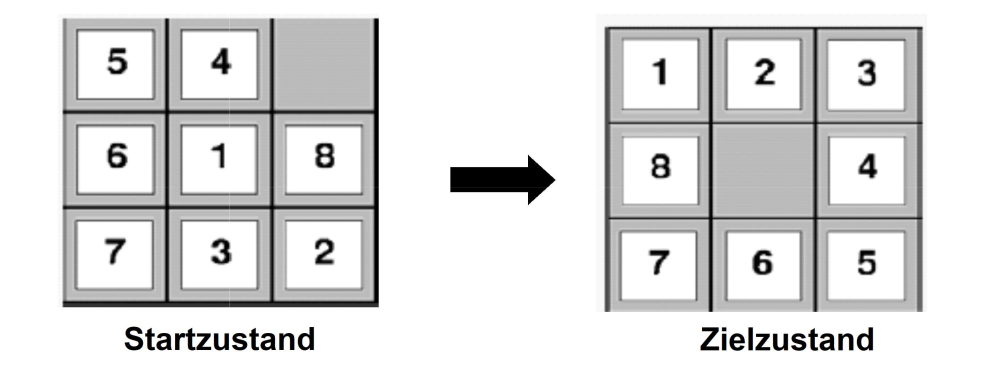
\includegraphics[width=0.8\textwidth]{figures/8er-puzzle.png}
    \caption{8er puzzle Start- und Zielzustand}
    \label{fig:8er-puzzle}
\end{figure}

\begin{itemize}
    \item Zust�nde: Lokalit�t der 8 Fliesen in eine der 9 Fl�chen plus eine freie Kachel
    \item Operatoren: Blank nach Links, Rechts, Auf, Ab 
    \item Ziel-test: Blank-Kachel in der Mitte
    \item Pfadkosten: jeder Schritt kostet eine Einheit
\end{itemize}

\subsection{Staubsauger-Roboter}

Vieles an der Implementierung dieses Roboters muss abstrahiert werden:
\begin{itemize}
    \item World States: Umfassen alle Aspekte der reelen Welt
    \item Problem States: Nur Aspekte der relevant f�r das Problem sind. Die Modellierung von diesen Aspekten erfolgt meist in Form \textbf{symbolisher} Beschreibungen. 
    \item Erstens m�ssen die m�glichen World States als Problem States dargestellt werden:
\end{itemize}

\begin{figure}[h!]
    \centering
    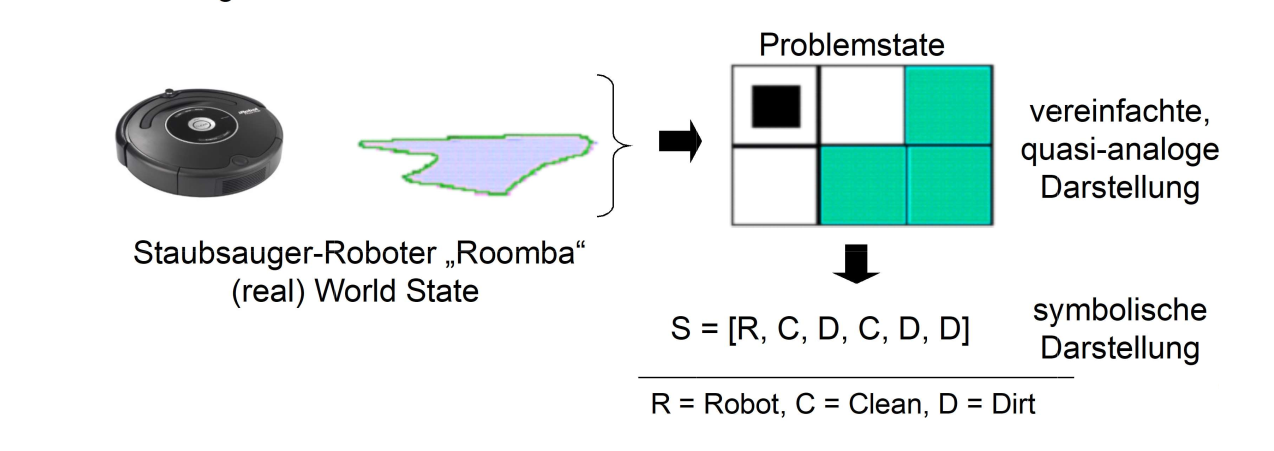
\includegraphics[width=0.8\textwidth]{figures/roomba-world-to-problem-states.png}
    \caption{Abbildung World States auf Problem States}
    \label{fig:roomba-abbildung}
\end{figure}


\section{Klassifikation von Problemen}

Es gibt viele Arten von Problemen und sie werden durch die Informationen des L�sers bestimmt. 

\paragraph{1. Probleme mit Einfach Zust�nden}

F�r den Probleml�ser ist klar, in welchem Zustand er sich befindet und was seine m�glichen Aktionen bewirken werden. Wie bereits im Roomba-Beispiel (Kap. \ref{section:roomba}) erw�hnt, kann dies als endlicher Zustandsautomat modelliert werden.

\paragraph{2. Probleme mit Mehrfach-Zust�nden}

Der genaue Zustand, in dem sich der Probleml�ser befindet, ist nicht bekannt, und der Probleml�ser wei� nicht, was seine Aktionen bewirken werden.

Anhand des Roomba-Beispiels: In dem Extremfall dass der Roomba keine Sensoren hat, kann er als mehrfaches Problem modelliert werden. In einem solchen Fall kann der Startzustand einer der Zust�nde S1 bis S8 sein (siehe Abb. \ref{fig:roomba-simplified}).

Eine m�gliche L�sung besteht darin, die Menge der aktuell m�glichen Zust�nde zu verwenden, um die Aktionen des L�sers zu bestimmen:

\begin{figure}[H]
    \centering
    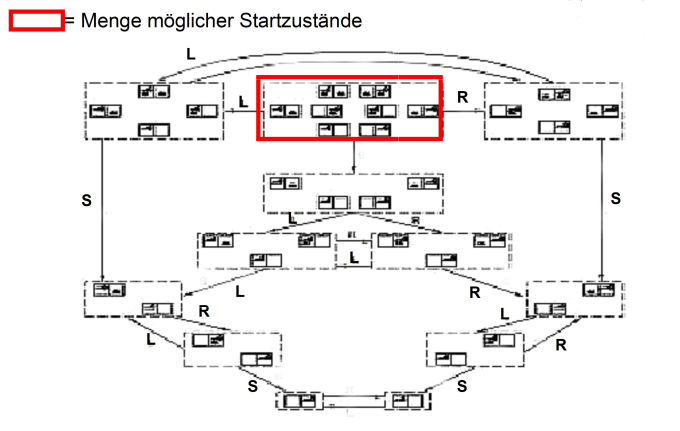
\includegraphics[width=0.8\textwidth]{figures/roomba-mehrfach.states.png}
    \caption{Staubsaugerwelt als Mehrfach-Problem}
    \label{fig:roomba-mehrfach-statemachine}
\end{figure}

\paragraph{3. Zufall-Probleme}

Der L�ser hat keine vollst�ndige Kenntnis einer sich st�ndig ver�ndernden Welt. Er kann nur die lokale Umgebung wahrnehmen.

Auch hier wieder das Roomba-Beispiel: Der Roboter befindet sich im Zustand S1 oder S3 und kann die Aktionen: Saugen, nach rechts fahren, Saugen ausf�hren. 

Der Roboter saugt und bewegt sich dann nach rechts. Wenn er aber sich vor der Bewegung im Zustand S3 befand, geht er zum Zustand S8 �ber. Er versucht dann zu saugen aber die Aktion schl�gt fehl, da in dem Zustand kein Staub vorhanden ist.

Um dieses Problem zu l�sen, ben�tigt der Roboter einen Sensor, der das Vorhandensein von Staub erkennt.

\begin{figure}[H]
    \centering
    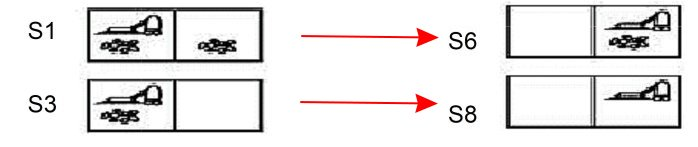
\includegraphics[width=0.8\textwidth]{figures/roomba-zufall.png}
    \caption{Roomba Zufallproblem}
    \label{fig:roomba-zufall}
\end{figure}

\paragraph{4. Explorations-Probleme}

Der L�ser hat keine Kenntnis von der Welt und muss seine Umgebung erkunden, um die m�glichen Zust�nde und die Auswirkungen seiner Aktionen zu erfahren.

Ein gutes Beispiel daf�r ist der Marsrover. Der Rover muss zun�chst Daten sammeln, um seine Umgebung kennenzulernen und eine Karte zu erstellen. Mit dieser Karte kann es dann erfolgreich die Pfadfindung durchf�hren.

\section{Rationaler autonomer Agent als Probleml�ser}

Ein rationaler autonomer Agent ist ein Wesen, das seine Welt permanent wahrnehmen und unabh�ngig reagieren kann.

\begin{figure}[H]
    \centering
    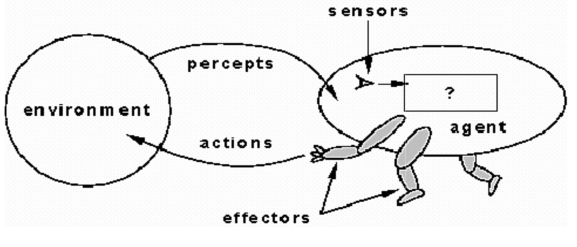
\includegraphics[width=0.8\textwidth]{figures/rational-agent.png}
    \caption{Rationaler autonomer Agent}
    \label{fig:rational-agent-diagram}
\end{figure}

Die Abbildung \ref{fig:rational-agent-diagram} veranschaulicht die Interaktion zwischen einem Agenten und seiner Umgebung unter Verwendung seiner Perzeptoren (PAGE = Percepts, Actions, Goals, Environment). 

\subsection{Einfaches Beispiel f�r einen rationalen autonomen Agenten}

\begin{figure}[H]
    \centering
    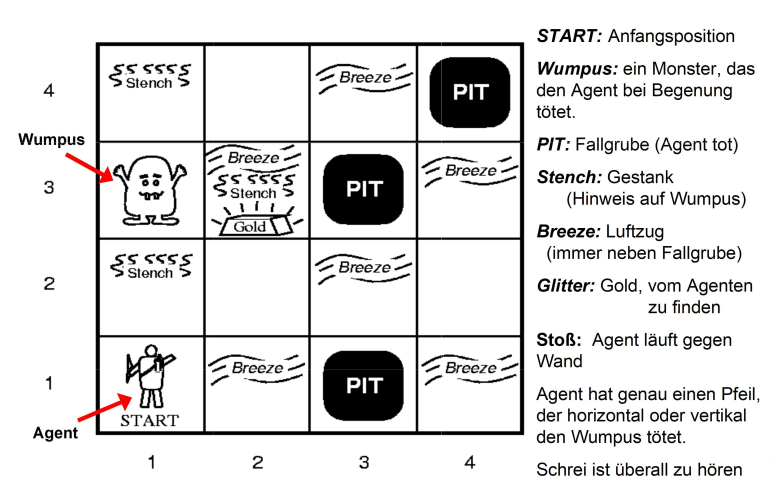
\includegraphics[width=0.8\textwidth]{figures/wumpus.png}
    \caption{Wumpus World}
    \label{fig:wumpus-example}
\end{figure}

Wumpus World ist eine H�hle mit 4/4 R�umen, die durch G�ngen verbunden sind. Es sind also insgesamt 16 R�ume miteinander verbunden. Es gibt einen wissensbasierten Agenten, der durch diese Welt gehen wird. Die H�hle hat einen Raum mit einem Monster namens Wumpus, das jeden frisst, der den Raum betritt. Wumpus kann vom Agenten erschossen werden, aber der Agent hat einen einzigen Pfeil. In der Welt von Wumpus gibt es mehrere endlose Lochr�ume und wenn ein Agent in ein Loch f�llt, wird er dort f�r immer gefangen sein. In einem der R�ume dieser H�hle befindet sich ein Haufen Gold. Das Ziel des Agenten ist es also, das Gold zu finden und aus der H�hle zu kommen, ohne in das Loch zu fallen oder von Wumpus gefressen zu werden. Der Agent wird belohnt, wenn er mit Gold herauskommt, und er bekommt eine Strafe, wenn er von Wumpus gefressen wird oder in ein Loch f�llt.

\paragraph{Umgebung von Wumpus World}
\begin{itemize}
    \item Ein 4x4-Raster von R�umen.
    \item Der Agent beginnt im Feld [1,1] und zeigt nach rechts.
    \item Standort von Wumpus und Gold werden zuf�llig ausgew�hlt, au�er Feld [1,1].
    \item Jedes Quadrat der H�hle kann mit Wahrscheinlichkeit 0,2 eine Grube sein, au�er dem ersten Quadrat
\end{itemize}

\paragraph{Eigenschaften von Wumpus World}
\begin{itemize}
    \item Die Welt ist teilweise beobachtbar, da der Agent nur die nahe Umgebung wahrnehmen kann, in der er sich befindet.
    \item Die Welt ist deterministisch, da die Auswirkungen aller Handlungen bekannt sind.
    \item Die Reihenfolge ist wichtig, also ist die Welt sequentiell.
    \item Die Welt ist statisch wie Wumpus und die Gruben bewegen sich nicht.
    \item Die Umgebung ist diskret.
    \item Einzelagentenumgebung (Wumpus wird nicht als Agent betrachtet, da er statisch ist)
\end{itemize}

\subsection{Arten von rationalen Agenten}

\paragraph{Reflex Agenten}

Ein Reflexagent ist eine Entit�t, die reaktiv ist und mit Sensoren arbeitet. Dieser Agent setzt sich keine Ziele und k�mmert sich nicht um die Auswirkungen seiner Handlungen.

\begin{figure}[H]
    \centering
    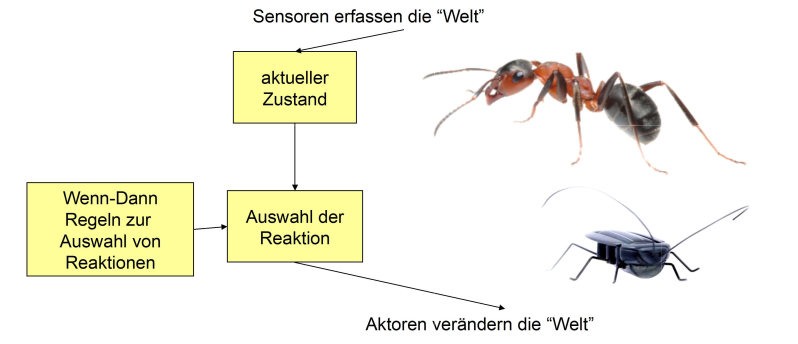
\includegraphics[width=0.8\textwidth]{figures/reflex-agent.png}
    \caption{Reflex-Agenten}
    \label{fig:reflex-agent}
\end{figure}

\paragraph{Ziel orientierter Agent}

Zielorientierte Agenten planen ihre Handlungen und antizipieren die Auswirkungen dieser Handlungen, um ihre Ziele zu erreichen.

\begin{figure}[H]
    \centering
    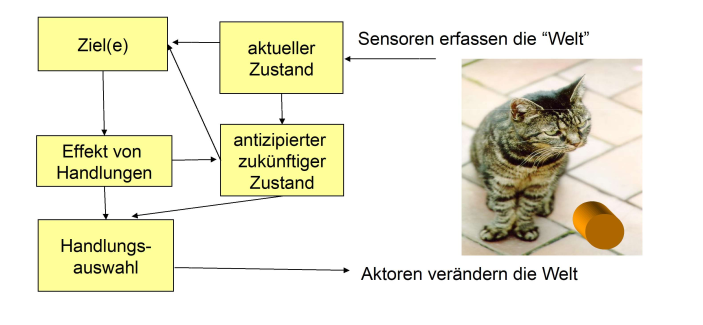
\includegraphics[width=0.8\textwidth]{figures/goal-oriented-agents.png}
    \caption{Ziel-orientierter Agenten}
    \label{fig:ziel-orientierter-agent}
\end{figure}

\newpage
\paragraph{Nutzen-orientierter Agent}

Ein nutzen-orientierter Agent w�gt die Kosten und Gewinne von Handlungen ab, um die Effektivit�t seiner Handlungen beim Erreichen eines Ziels zu maximieren.

\begin{figure}[H]
    \centering
    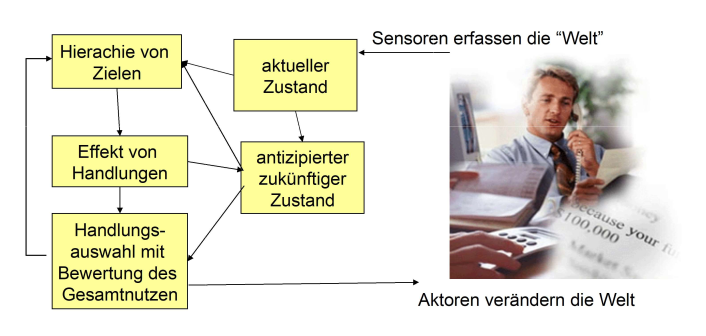
\includegraphics[width=0.8\textwidth]{figures/nutzen-orientierter-agent.png}
    \caption{Nutzen-orientierter Agenten}
    \label{fig:nutzen-orientierter-agent}
\end{figure}

\paragraph{Lern-f�higer Agent}

Diese Art von Agent ist in der Lage, die Effekte seiner Handlungen zu lernen, um seine Ziele besser zu erreichen, indem er seine Handlungen effektiver ausw�hlt.

\begin{figure}[H]
    \centering
    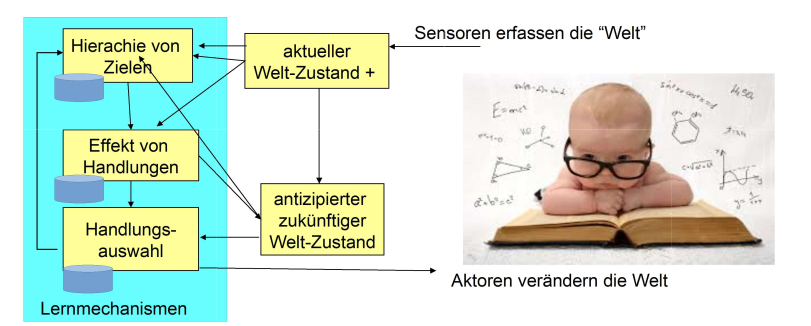
\includegraphics[width=0.8\textwidth]{figures/lern-agent.png}
    \caption{Lern-f�higer Agenten}
    \label{fig:lernen-agent}
\end{figure}

\paragraph{Emotionaler Agent}

Dieser Agent verwendet neben rationalem Denken eine emotionale Bewertung, um reale menschliche Entscheidungsprozesse besser zu simulieren.

\begin{figure}[H]
    \centering
    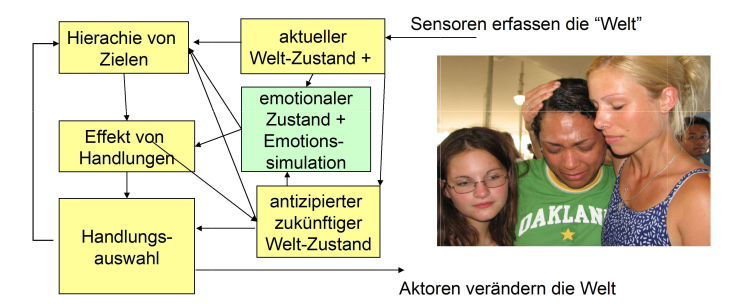
\includegraphics[width=0.8\textwidth]{figures/emotionaler-agent.png}
    \caption{Emotionaler Agent}
    \label{fig:emo-agent}
\end{figure}

\paragraph{Kreativer Agent}

Dieser Agent hat die F�higkeit, neue Aktionen zu entwickeln, um neue Wege zur L�sung von Problemen zu schaffen, die nicht vorprogrammiert waren.

\begin{figure}[H]
    \centering
    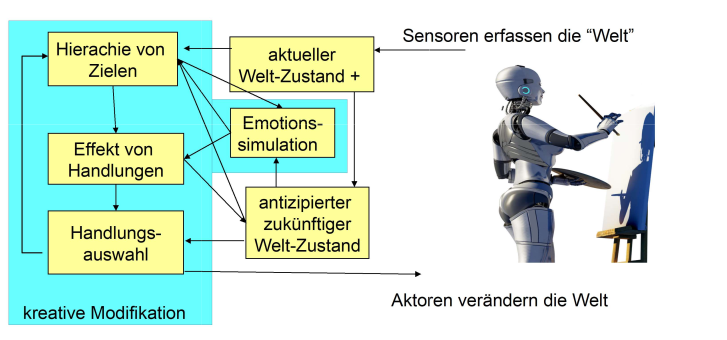
\includegraphics[width=0.8\textwidth]{figures/creative-agent.png}
    \caption{Kreativer Agent}
    \label{fig:creative-agent}
\end{figure}


\paragraph{Kooperative Agenten}

Eine Situation, in der mehrere Agenten zusammenarbeiten, um komplexe Aufgaben zu l�sen. Dies erfordert die Modellierung kooperativer Verhaltensstrategien und das Verst�ndnis der Absichten anderer Agenten.

\begin{figure}[H]
    \centering
    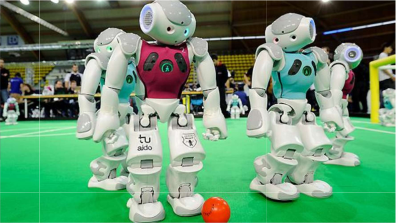
\includegraphics[width=0.8\textwidth]{figures/robocup.png}
    \caption{Robocup competition: Cooperative agents}
    \label{fig:coop-agent}
\end{figure}